\usepackage{hyperref}

%%%%%%%%%%%%%%%%%%%%%%%%%%%%%%%%%%%%%%%%%%%%%%%%%%%%%%%%%%%%%%%%%
%  _____   ____  _____                                          %
% |_   _| /  __||  __ \    Institute of Computitional Physics   %
%   | |  |  /   | |__) |   Zuercher Hochschule Winterthur       %
%   | |  | (    |  ___/    (University of Applied Sciences)     %
%  _| |_ |  \__ | |        8401 Winterthur, Switzerland         %
% |_____| \____||_|                                             %
%%%%%%%%%%%%%%%%%%%%%%%%%%%%%%%%%%%%%%%%%%%%%%%%%%%%%%%%%%%%%%%%%
%
% Project     : LaTeX doc Vorlage für Windows ProTeXt mit TexMakerX
% Title       : 
% File        : grundlagen.tex Rev. 00
% Date        : 7.5.12
% Author      : Remo Ritzmann
% Feedback bitte an Email: remo.ritzmann@pfunzle.ch
%
%%%%%%%%%%%%%%%%%%%%%%%%%%%%%%%%%%%%%%%%%%%%%%%%%%%%%%%%%%%%%%%%%

\chapter{Technical and Theoretical Foundation}
\label{chap.grundlagen}
\chaptermark{Foundations}
\section{Reinforcement Learning}\label{reinforcementlearning}
\subsection*{Basic Definitions}\label{basic_rl_definitions}
In recent years, major progress has been achieved in the field of reinforcement learning (RL) \cite{mnih2013playing,alphazero,hideandseek}.
In RL, an agent learns to perform a task by interacting with an environment $\mathcal{E}$ as displayed in \autoref{fig:rl_overview}. On every timestep $\mathcal{t}$ the agent $\mathcal{a}$ needs to take an action $\mathcal{u}$. The selection of this action $\mathcal{u}$ is based on the current observation $\mathcal{s}$. The success of the agent is measured by reward $\mathcal{R}$ received. If the agent does well, it receives positive reward from the environment, if it does something bad, there is no or negative reward.
\begin{figure}[H]
	\centering
	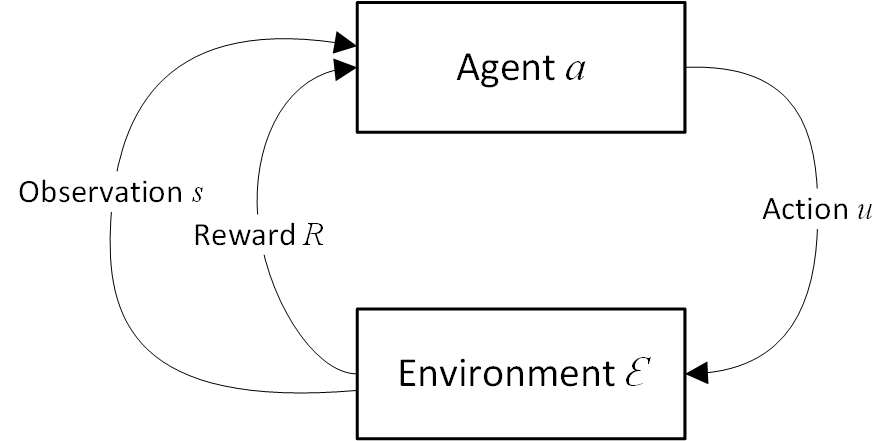
\includegraphics[width=250pt]{images/rl_overview.png}
	\caption{Reinforcement learning overview}
	\label{fig:rl_overview}
\end{figure}
The goal of the agent is now to take an action that maximizes the expected reward for all future timesteps $\EX[\mathcal{R}_{t+1}+\mathcal{R}_{t+1}+\mathcal{R}_{t+1}+...|\mathcal{s}_{t}]$ given the current observation $\mathcal{s}$.\\
This estimation should be as close as possible to the sum of actually received rewards. Often, these received rewards are discounted with a constant factor $\mathcal{\gamma}$ to the power of timestep $\mathcal{t}$. With $\mathcal{\gamma}$ being something slightly less than 1, this accounts for the fact that rewards far in the future are hard to estimate.
The current observation $\mathcal{s}_{t}$, also known as the current state is used to determine which action $\mathcal{u}$ to take next. An agent can observe its environment either fully or partially. The cycle of taking actions and receiving a new state is repeated until the environment has reached a terminal state. Each rollout of such an environment is called an episode.
\subsection*{Value Based vs. Policy Gradient Based Methods}\label{value_policy_based_methods}
Reinforcement learning methods are categorized into value-based methods and policy gradient-based methods \cite{tdlearning},\cite{policygradient}. Those variants differ on how they select an action $\mathcal{u}$ from a given state $\mathcal{s}$.\\
Value-based RL algorithms work by learning a value function $\mathcal{V(s)}$ through repeated rollouts of the environment. $\mathcal{V(s)}$ aims to estimate the future expected reward for any given state $\mathcal{s}$ as precisely as possible. Using this approximation $\mathcal{V(s)}$ we can now select the action $\mathcal{u}$ that takes the agent into the next state $\mathcal{s}_{t+1}$ with the highest expected future reward. This estimation $\mathcal{V(s)}$ is achieved by either a lookup table for all possible states or a function approximator. In this work, we solely focus on the case that $\mathcal{V(s)}$ is implemented in form of a neural network as function approximator. To train the neural network, we try to minimize the squared difference between the estimated reward $\mathcal{V(s)}$ and the actual reward:
\begin{gather*}
loss_{value}=(\mathcal{R}-\mathcal{V(s)})^2
\end{gather*}
In some value-based algorithms such as Deep Q-Networks \cite{mnih2013playing}, a $\mathcal{Q(s,u)}$-function is used. This function tries to estimate the expected future reward on taking action $\mathcal{u}$ from the given state $\mathcal{s}$.\\
The second category of reinfocement learning algrithms are the so called policy gradient based methods. These methods aim to aquire a stochastic policy $\pi$ that maximizes the expected future reward $\mathcal{R}$ by taking actions with certain probabilities. Taking actions based on probabilities solves an important issue of value based methods, which is, that by taking greedy actions with respect to state  $\mathcal{s}$, the agent might not explore the whole state space and misses out on better ways to act in the environment.

\subsection*{Asynchronous Advantage Actor Critic Algorithm (A3C)}\label{a3c_intro}
The progress in RL has led to algorithms that combine value based and policy gradient based methods, generally known as actor-critic algorithms. The \textit{asynchronous advantage actor critic algorithm} (A3C), developed by Mnih et al. \cite{a3c} fits into this category. It uses both a policy $\pi$ and a value function $\mathcal{V(s)}$.
Both are usually seperate function approximators (neural networks in our case).
\begin{itemize}
	\item The \textbf{actor} can be seen as the policy $\pi$, that selects the action $\mathcal{u}$ based on a state $\mathcal{s}$.
	\item The \textbf{critic} is the value function $\mathcal{V(s)}$ that estimates, how much reward can be expected from a certain state on.
\end{itemize}
To enhance the process of learning policy $\pi$, the policy loss gets multiplied by the difference between actually received reward $\mathcal{R}$ and the estimated future reward $\mathcal{V(s)}$. This difference is called the advantage $\mathcal{A}$.
\begin{gather*}
\mathcal{A}=\mathcal{R}-\mathcal{V(s)}
\end{gather*}
This advantage is then used to update the policy.
\begin{gather*}
loss_{policy}=log \pi(s_{t})*\mathcal{A}
\end{gather*}
For actions where the received reward $\mathcal{R}$ exceeds the expected reward $\mathcal{V(s)}$ the policy update gets multiplied by a positive advantage. Therefore, the update of the neural network gets adjusted into a direction that favors the experienced actions based on the seen states.\\
What makes A3C different from other actor-critic algorithms is, that it can be used in a distributed way. Many workers work at the same time on a centralized model. How we take advantage of this features is discussed in \nameref{dist_architecture}.

\section{The Flatland Rail Environment}\label{flatland_intro}
The Flatland environment is a virtual simulation environment provided by the Swiss Federal Railway SBB and the crowdsourcing platform AICrowd.
The goal of this environment is to act as a simplified simulation of real train traffic. The current state of the simulation is shown in \autoref{fig:screenshot_flatland}.
\begin{figure}[H]
	\centering
	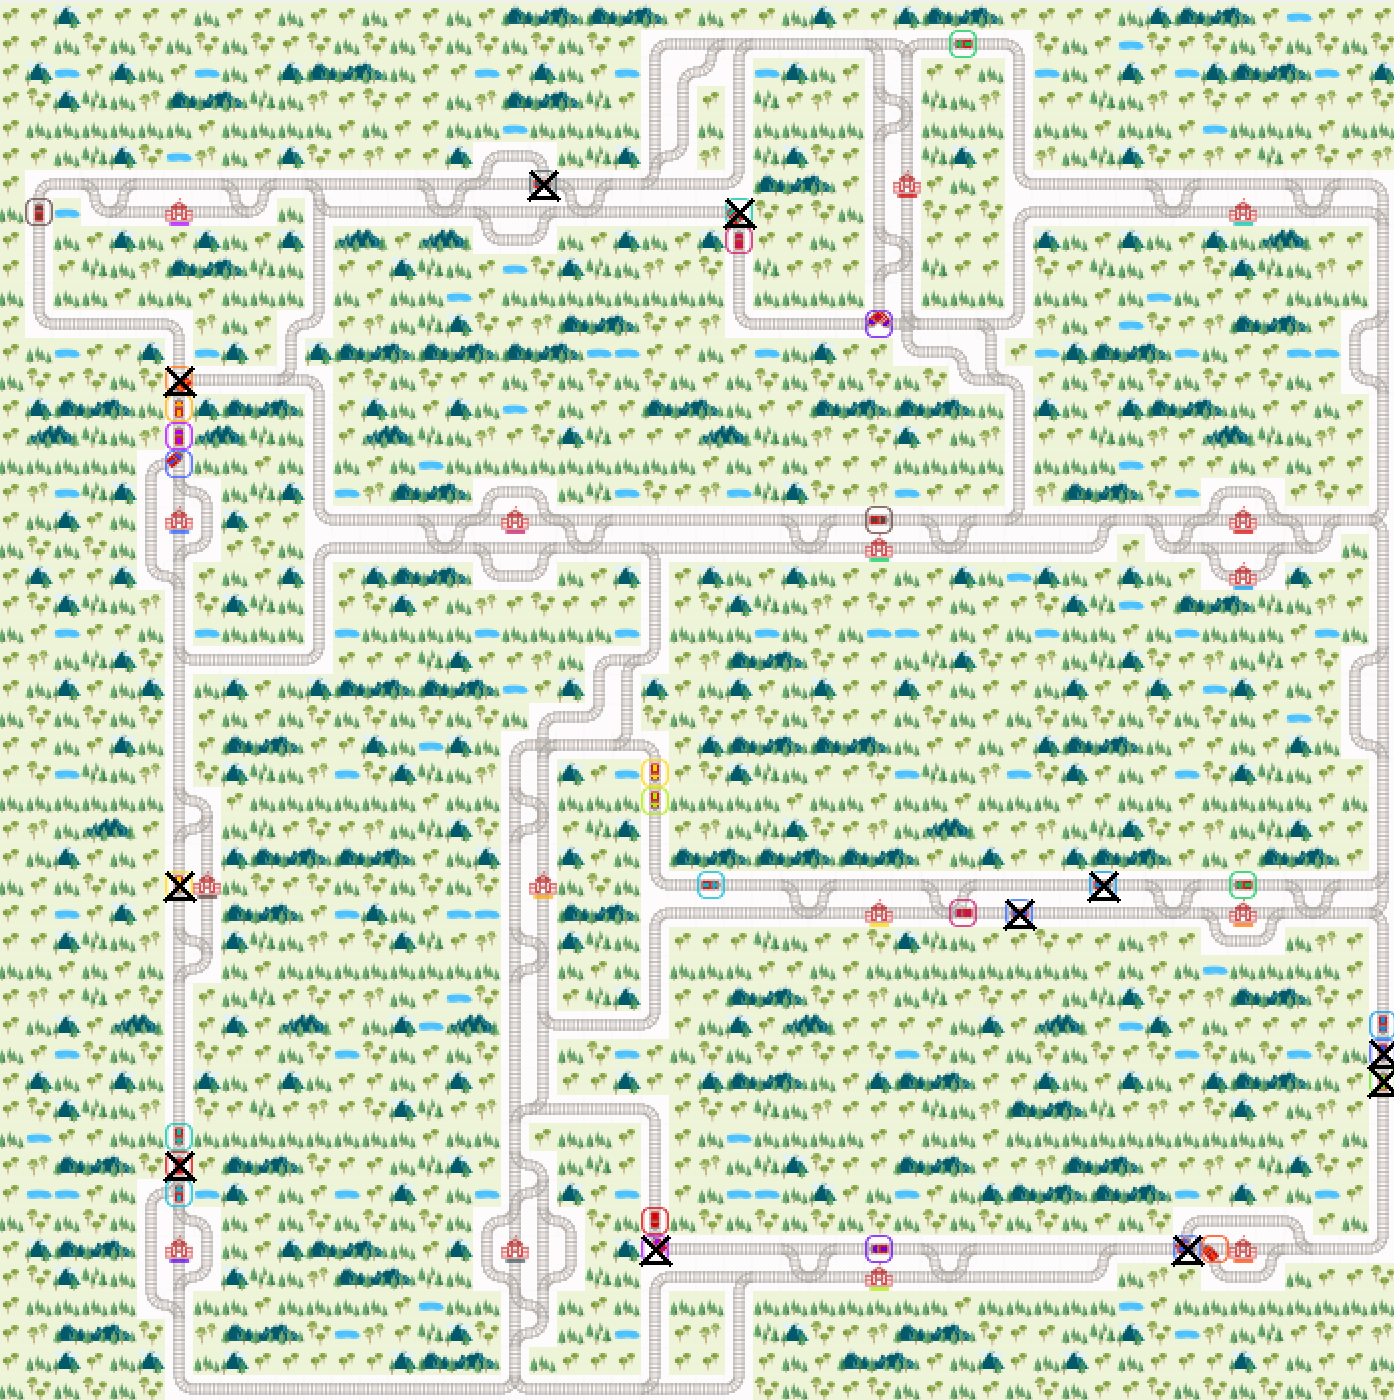
\includegraphics[width=300pt]{images/screenshot_flatland.png}
	\caption{Screenshot from a running Flatland environment.}
	\label{fig:screenshot_flatland}
\end{figure}
Using Flatland, we can train RL algorithms to control the actions of trains, based on observations on the grid. Flatland has a discrete structure in both its positions and its timesteps. The whole rail grid is composed out of squares that can have connections to neighbouring squares. In certain squares, the rails splits into two rails. On those switches, the agent has to make a decision which action it wants to take. Dependent on the type of switch, there are different actions available compare \autoref{fig:switches_flatland}.
\begin{figure}[H]
	\centering
	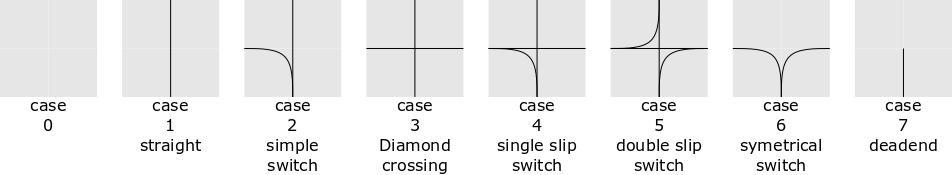
\includegraphics[width=300pt]{images/transition_nips_proposal.png}
	\caption{Possible switches in the Flatland environment from \cite{flatland_docu}.}
	\label{fig:switches_flatland}
\end{figure}
An exception poses switches that are approached from a side that does not allow to take an action, e.g. approaching a \textit{case 2} switch from the north side.
All rail parts, independent of if it is a switch also allow to take the actions to do nothing (remain halted, or keep riding), to go forward or to brake.
The action space is therefore defined by:
\begin{gather*}
U = \{ \text{do nothing, go left, go forward, go right, brake} \}
\end{gather*}
It is important to note that trains do not have the ability to go backwards and therefore need to plan ahead to avoid getting stuck. To learn which actions to take, the agents have to learn to adapt to an unknown environment due to the fact that the environments are randomly generated and differ on each episode. Depending on the given parameters, the size and complexity of the grid can be adjusted. This allows for dynamically changing the difficulty for the agents.\\
The goal of each agent is to reach an assigned target train station as fast as possible. Agents that reach this destination are removed from the grid which means, they can no longer obstruct the path of other trains.

\subsection*{Observations}\label{observations}
The Flatland environment allows to create observation builders to observe the environment for each agent. While it is possible to observe the whole grid, this does usually not make sense due to the fact that many parts of the rail grid are not relevant to a single train. Flatland offers by default two different observation builders.\\\\
\textbf{GlobalObsForRailEnv} creates three arrays with the dimensions of the rectangular rail grid. The first array contains the transition information of the rail grid. For each cells, there are 16 bit values, 4 bit for each possible direction a train is facing.\\\\
\textbf{TreeObsForRailEnv} creates a graph with sections of the grid as nodes from the perspective of the train.
This means, only the switches which the train is actually able to take define a single node. As an example, a train on a \textit{case 0} switch heading from north to south is not able to make a decision on this switch and therefore, the TreeObservation does not put the sections before and after the switch into two different nodes but just into a single node.\\
The nodes of the tree observation offer a number of fields that allow to select specific features to create numeric input vectors for function approximator such as neural networks. The tree observation builder offers 14 distinct features for each rail section. This includes:
\begin{itemize}
	\item Distance until own target encountered: Cell distance to the own target railway station. Infinitiv if target railway station for agent is not in this section.
	\item Distance to other agent encountered: Cell distance to the next other agent on this section.
	\item Distance to next branch: The length of this section.
	\item Min. distance to target: The minimal cell distance to the target after this section is finished.
	\item Child nodes: The nodes the agent is able to take after this section ends. Each child node is associated with a direction (left, forward, right).
\end{itemize}
\subsection*{Agent Evaluation}\label{rl_agent_eval}
AICrowd and SBB provide a system for agent evaluation. This system evaluates the policy on a number of unknown environments and outputs the percentage of agents that reached their assigned destination as well as the received reward while doing so. The evaluation reward scheme is thereby as follows \cite{flatland_faq}:
\begin{gather*}
R_{t}= 
\begin{cases}
-1,				& \text{if } s_{t} \text{ is not terminal}\\
10,             & \text{otherwise}
\end{cases}
\end{gather*}
The difficulty of the evaluation level does differ between round 1 and round 2. While round 1 offered many connecting rails between the starting position and the assigned target of an agent, round 2 has more sparse connections and usually only provides 2 to 4 rails between cities. The concept of cities has been added in round 2. Those differences can be clearly seen in \autoref{fig:eval_comp} with the densly connected environment for round 1 versus the sparsly connected environment for round 2. 
\begin{figure}[H]
	\centering
	\begin{subfigure}{.5\textwidth}
		\centering
		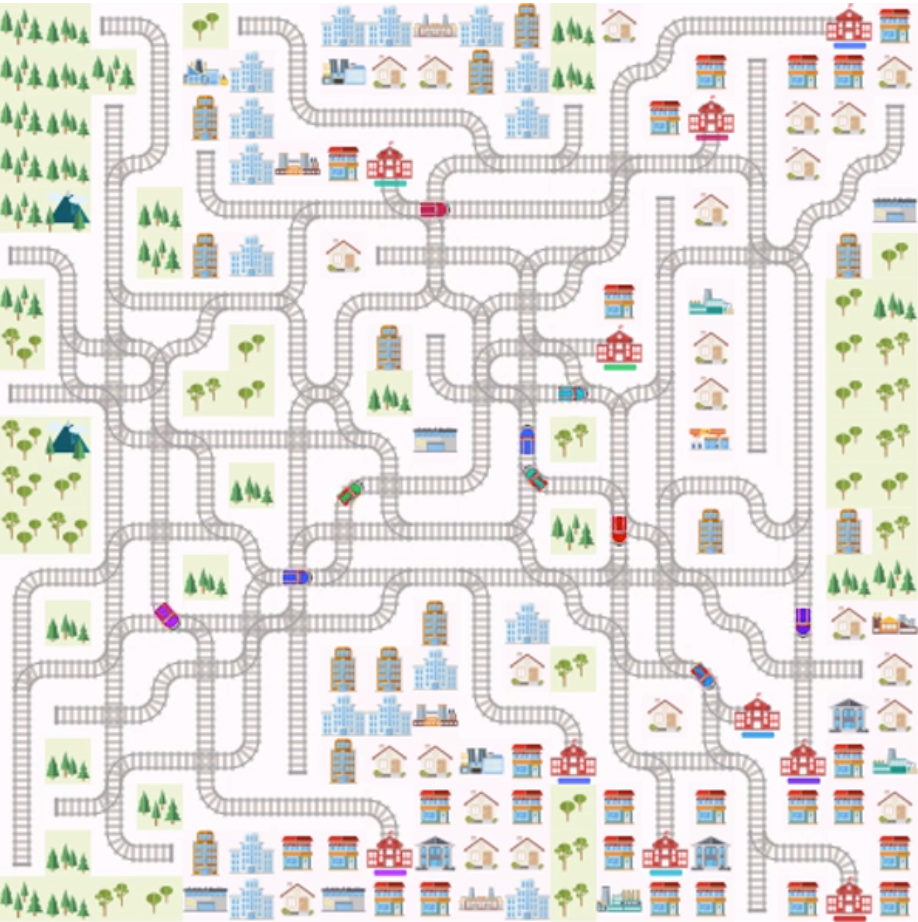
\includegraphics[width=200pt]{images/example_eval_round1.png}
		\caption{Evaluation round 1.}
		\label{fig:eval_round1}
	\end{subfigure}%
	\begin{subfigure}{.5\textwidth}
		\centering
		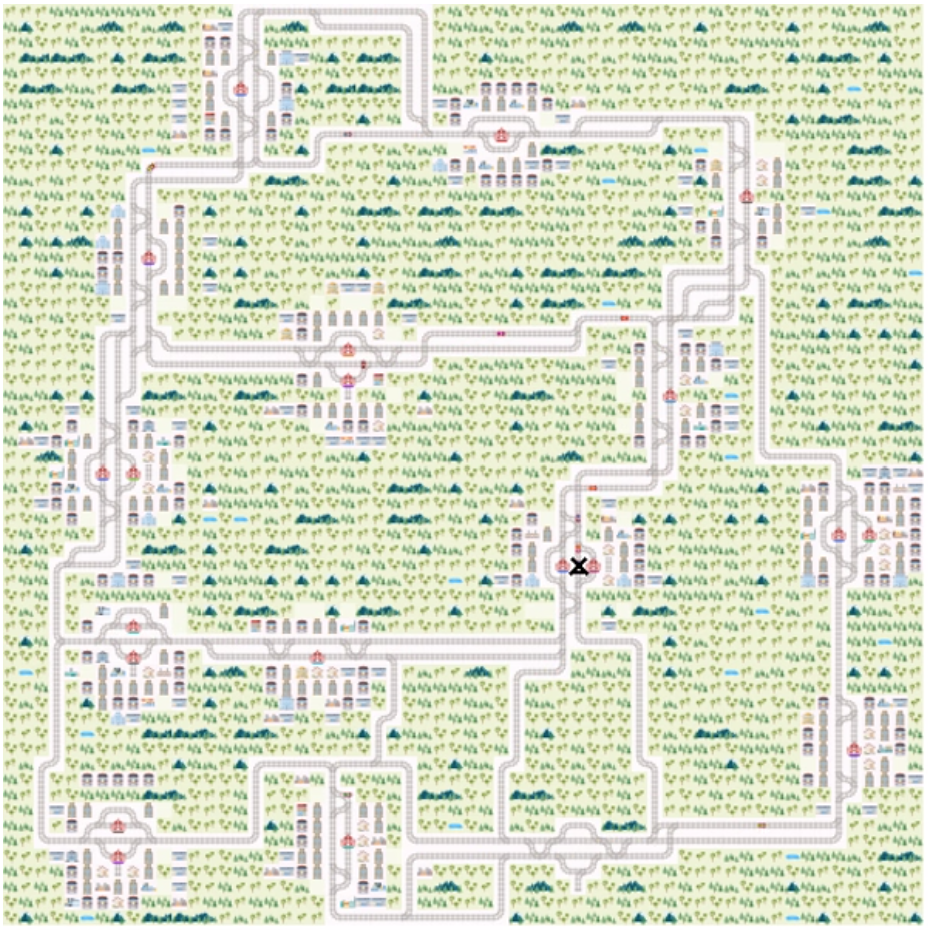
\includegraphics[width=200pt]{images/example_eval_round2.png}
		\caption{Evaluation round 2.}
		\label{fig:eval_round2}
	\end{subfigure}
	\caption{Comparison between two screenshots from evaluation environments from Flatland round 1 and round 2.}
	\label{fig:eval_comp}
\end{figure}

